	%====================================================================================================
	% ?????
	%====================================================================================================
	% TCC
	%----------------------------------------------------------------------------------------------------
	% Autor				: Jasane Schio
	% Orientador		: Gedson Faria
	% Co-Orientador		: Angelo Darcy
	% Instituição 		: UFMS - Universidade Federal do Mato Grosso do Sul
	% Departamento		: CPCX - Sistema de Informação
	%----------------------------------------------------------------------------------------------------
	% Data de criação	: 01 de Outubro de 2015
	%====================================================================================================
	%descrever problemas e as solucoes encontradas
	\definecolor{dkgreen}{rgb}{0,0.6,0}
	\definecolor{gray}{rgb}{0.5,0.5,0.5}
	\definecolor{mauve}{rgb}{0.58,0,0.82}
	
	\lstset{frame=tb,
		language=C++,
		aboveskip=3mm,
		belowskip=3mm,
		showstringspaces=false,
		columns=flexible,
		basicstyle={\small\ttfamily},
		numbers=none,
		numberstyle=\tiny\color{gray},
		keywordstyle=\color{blue},
		commentstyle=\color{dkgreen},
		stringstyle=\color{mauve},
		breaklines=true,
		breakatwhitespace=true,
		tabsize=3
	}
	\chapter{Desenvolvimento} 
	
			Para o desenvolvimento foi escolhida a biblioteca OpenCV por ser OpenSource, multiplataforma, conter uma grande quantidade de métodos e algoritmos já implementados	e pelo seu rápido desempenho de máquina.
			A linguagem escolhida para o desenvolvimento foi o C++ pois é uma linguagem de programação compilada, o que torna sua execução mais rápida que as linguagem interpretadas, dando ao sistema uma performance em tempo satisfatório.	
\section{Tecnologias Usadas}
Para realização deste trabalho, irei utilizar a biblioteca de processamentos de imagens conhecida como OpenCV: Open Source Computer Vision Library. O trabalho será elaborado na linguagem C++, com uso do framework Qt para sua interface gráfica.
Os passos detalhados do projeto e seu desenvolvimento estará presente no Capítulo de Metodologia.
\begin{description}
	\item[OpenCV] Lançado em 1999 pela Intel\cite{Culjak:2012}, com objetivo de ser otimizada, portável e com um grande número de funções, o Open Source Computer Vision Library, OpenCV, se tornou se tornou uma ferramenta que possui mais de 2500 algoritmos e 40 mil pessoas em seu grupo de usuários\cite{Culjak:2012}. Já possui interface para as linguagens C++, C, Python e Java além de suporte para as principais plataformas com Windows, Linux, Mac OS, iOS e Android. A biblioteca lida tanto com imagens em tempo real, como vídeos e imagens estáticas.
	
	\item[Qt] Qt é um framework de desenvolvimento de aplicações multiplataforma. Entre suas funcionalidades está a possibilidade de criar interfaces gráficas diretamente em C++ usando seu módulo Widgets.
	
	\item [C++] A linguagem de programação C++ foi projetado por Bjarne Stroustrup para fornecer eficiência e flexibilidade da linguagem C para programação de sistemas. A linguagem evoluiu a partir de uma versão anterior chamado C com Classes, o projeto C com Classes durou entre 1979 e 1983 e determinou os moldes para o C++. A linguagem foi oficialmente lancada em 1986\cite{Stroustrup:1996}.
\end{description}

\section{Projeto}
\subsection{Organização do Projeto}
	 O projeto foi desenvolvido seguindo o paradigma de programação Orientada à Objetos, esse paradigma baseia-se na utilização de objetos individuais para criação de um sistema maior e complexo. A IDE usada para o desenvolvimento foi a QT Creator, esta separada o projeto em três pastas: Headers, Sources e Forms. Na pasta Headers estão os arquivos de cabeçalho(.h), onde estão as declarações dos métodos e variáveis usados nas classes  executáveis. Já na pasta Sources estão os arquivos fonte(.cpp), são nesses arquivos que os métodos declarados nos arquivos da pasta Header são implementados. Na pasta Forms está o arquivo de interface gráfica(.ui) que é usado no projeto para ser a ponte entre o usuário e as funções do sistema.
	 
	\begin{figure}[!h]
		\centering
		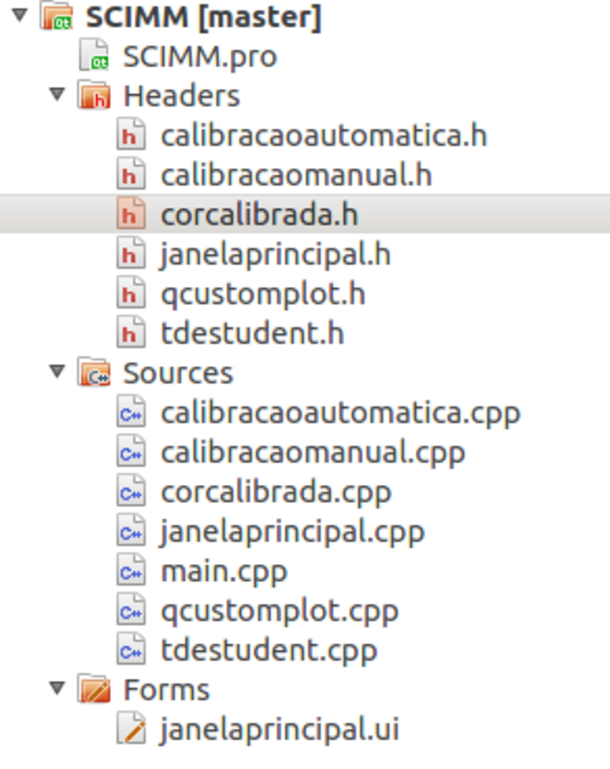
\includegraphics[width=0.2\textwidth]{organizacaoProjeto.pdf}
		\caption{Organização das pastas do projeto}
		\label{Organizacao do Projeto}
	\end{figure}
	Com exceção do arquivo fonte main, cada arquivo de cabeçalho possui um arquivo fonte correspondente, formando assim um objeto, todo objeto é uma classe mas nem toda classe forma um objeto. As classes desenvolvidas no projeto são: Calibração, scimm\_cor e janelaprincipal.
%Para melhor entendimento da interação entre as classes a figura 3.2 trás o diagrama de classes do projeto.

\subsection{Classes}
\subsubsection{main}
 Esta é o que se chama de \textit{ponto de entrada} em programação. \textit{Ponto de entrada} é onde o sistema operacional ira iniciar a execução do sistema desenvolvido. Esta classe possui somente o método \textbf{main} e este instancia e inicia o objeto \textbf{JanelaPrincipal} que apresenta a interface gráfica para interação com o usuário.
 
\subsubsection{JanelaPrincipal}
É uma classe-objeto que utiliza da implementação de objetos QWidget e suas subclasses disponíveis pelo framework Qt, para a criação de uma interface gráfica que faz a interação com o usuário. Todos os métodos presentes nessa classe são para utilização gráfica, comportamento de botões e menu de seleção, para a comunicação com a classe de calibração.	

\subsubsection{Calibracao}
 É classe que contem todos os métodos e variáveis usados no processo de calibração, é também dentro dessa classe que são feitas todos os tipos de manipulação em imagem.
 
Os métodos contidos na classe Calibração são:
	\begin{description}

\item Iniciar: Método onde é instanciado o objeto que faz referencia à \textbf{JanelaPrincipal}, para ser usado quando houver necessidade de comunicação com a interface que não seja por meio de retorno, este método também é onde se inicializa o a câmera, a partir do id contido na interface, e se verifica se a mesma esta disponível.


\item ConfigurarCamera: Método onde a imagem de exibição é ajustando o tamanho da tela a ser usada durante a detecção de objetos, além do ajuste de brilho e contraste para tornar mais nítido os contornos durante a detecção de objetos.	
	
  \item ReconhecerFundoExtrairObjetos: Método onde se utiliza o algoritmo de subtração de fundo para identificar, inicialmente, o campo e uma vez identificado se separa os objetos que não fazem parte do fundo inicial, a extração dos objetos. A extração dos objetos gerando uma imagem \textit{máscara} que sera usada na detecção dos objetos para que a mesma ser executada com mais precisão, uma vez que os objetos coloridos eram os únicos que não fazem parte da imagem inicial, o fundo.
  
 
	\item Calibrar: Método onde se a imagem atual da câmera é obtida e ajustada de acordo com os parâmetros estabelecidos no método \textbf{ConfigurarCamera} e iniciado o método \textbf{DetectarObjetos}. Uma vez que os objetos foram identificados se faz o uso do método \textbf{Calcular}  para serem analisados os valores de cada pixel de cada objetos e estes classificados de acordo com as cores pré definidas pelo sistemas. Uma vez terminado o processo de calibração é exibida na tela para o usuário os objetos da cor que esta selecionada no menu de cores.			
		
	\item DetectarObjetos: Método onde serão aplicados filtros de diminuição de ruido, detectadas as bordas existentes na imagem, detectados os objetos a partir das bordas contidas na imagem, o aumento da precisão do contorno dos objetos e diminuição do tamanho do objeto de acordo com a porcentagem de borda a ser eliminada. 

	\item ObterPorcentagem: Método simples para devolver a porcentagem de um valor, ao ser informado o valor e a porcentagem escolhida.
		
		\item Calcular: Método onde cada pixel pertencente à cada um dos objetos encontrados é analisado, seu valor H é categorizado de acordo com as cores pre-definidas no sistema e adicionado à cor correspondente.
		O algoritmo de categorização:
 
	
		\end{description}	

\subsubsection{SCIMM\_COR}
	Classe de cor utilizada do sistema. Onde são salvos os valores máximos e mínimos de HSV. Possui seis valores, um mínimo e um máximo para H, S e V. 


\section{O Sistema}

		 O sistema consiste na apresentação da \textbf{interface gráfica} ao usuário. A \textbf{interface gráfica} que por sua vez oferece as duas possibilidades ao usuário, de acordo com o tipo de calibração escolhido o sistema inicia a rotina de calibração referente. Apos a execução de toda o sistema é finalizada, como mostra o diagrama de fluxo na Figura \ref{FlowCHart}.
		
		\begin{figure}[H]
			\centering
			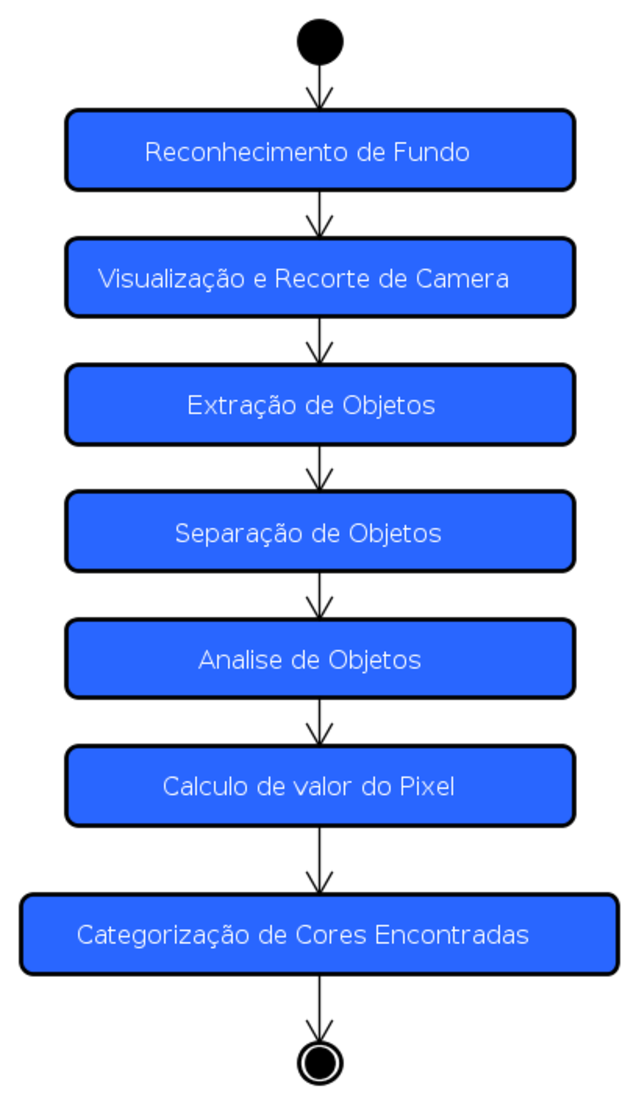
\includegraphics[width=0.45\textwidth]{FluxodoSistema.pdf}
			\caption{Diagrama de Fluxo}
			\label{FlowCHart}
		\end{figure}			
	 
		A rotina de calibração automática possui cinco etapas e os mesmos possuem o mínimo de interação possível do usuário. Nas subseções à seguir explicarei detalhadamente cada uma das etapas do processo de calibração automática
		\subsection{1ª Etapa - Configuração de Ca mera}
		

Para melhor desempenho do algoritmo de detecção de objetos, a imagem é recortada somente para o tamanho necessário do campo. O recorte de imagem foi feito utilizando a função setMouseCallback para possibilitar a interação do usuário na imagem por meio do mouse, sua utilização é dada da seguinte maneira:
\begin{center}
\centering \textit{ cv::setMouseCallback(src\_window,mouseHandler,0);}
\end{center}
Tem como primeiro parâmetro \textbf{src\_windows} que indica a janela na qual a função recebera a interação,  o segundo, \textbf{mouseHandler}, indica a função na qual esta implementada a interação e o ultimo parâmetro, \textbf{0}, indica parâmetros opcionais, neste caso não usaremos nenhum então foi usado o numero 0.
Dentro da função \textbf{mouseHandler} são identificados os pontos iniciai e final da seleção na tela e utilizada a função \textit{rectangle} para demarcar a seleção na tela. A utilização da função \textit{rectangle} completa fica da seguinte maneira:
\begin{center}
\centering \textit{ cv::rectangle(frameA, point1, point2, CV\_RGB(255, 0, 0), 2, 5, 0);}
\end{center}
A função recebe os parâmetros \textbf{frameA} indicando a imagem na qual será demarcada a área selecionada, depois o parâmetro \textbf{point1} que é o ponto inicial de seleção na imagem, \textbf{point2} que é o ponto final da seleção. \textbf{CV\_RGB(255, 0, 0)} que indica a cor da demarcação, \textbf{2} indicando a espessura da demarcação, \textbf{5} que significa o tipo de linha a ser utilizado na demarcação e \textbf{0} que é o numero de bits fracionários.

\begin{figure}[H]
			\centering
			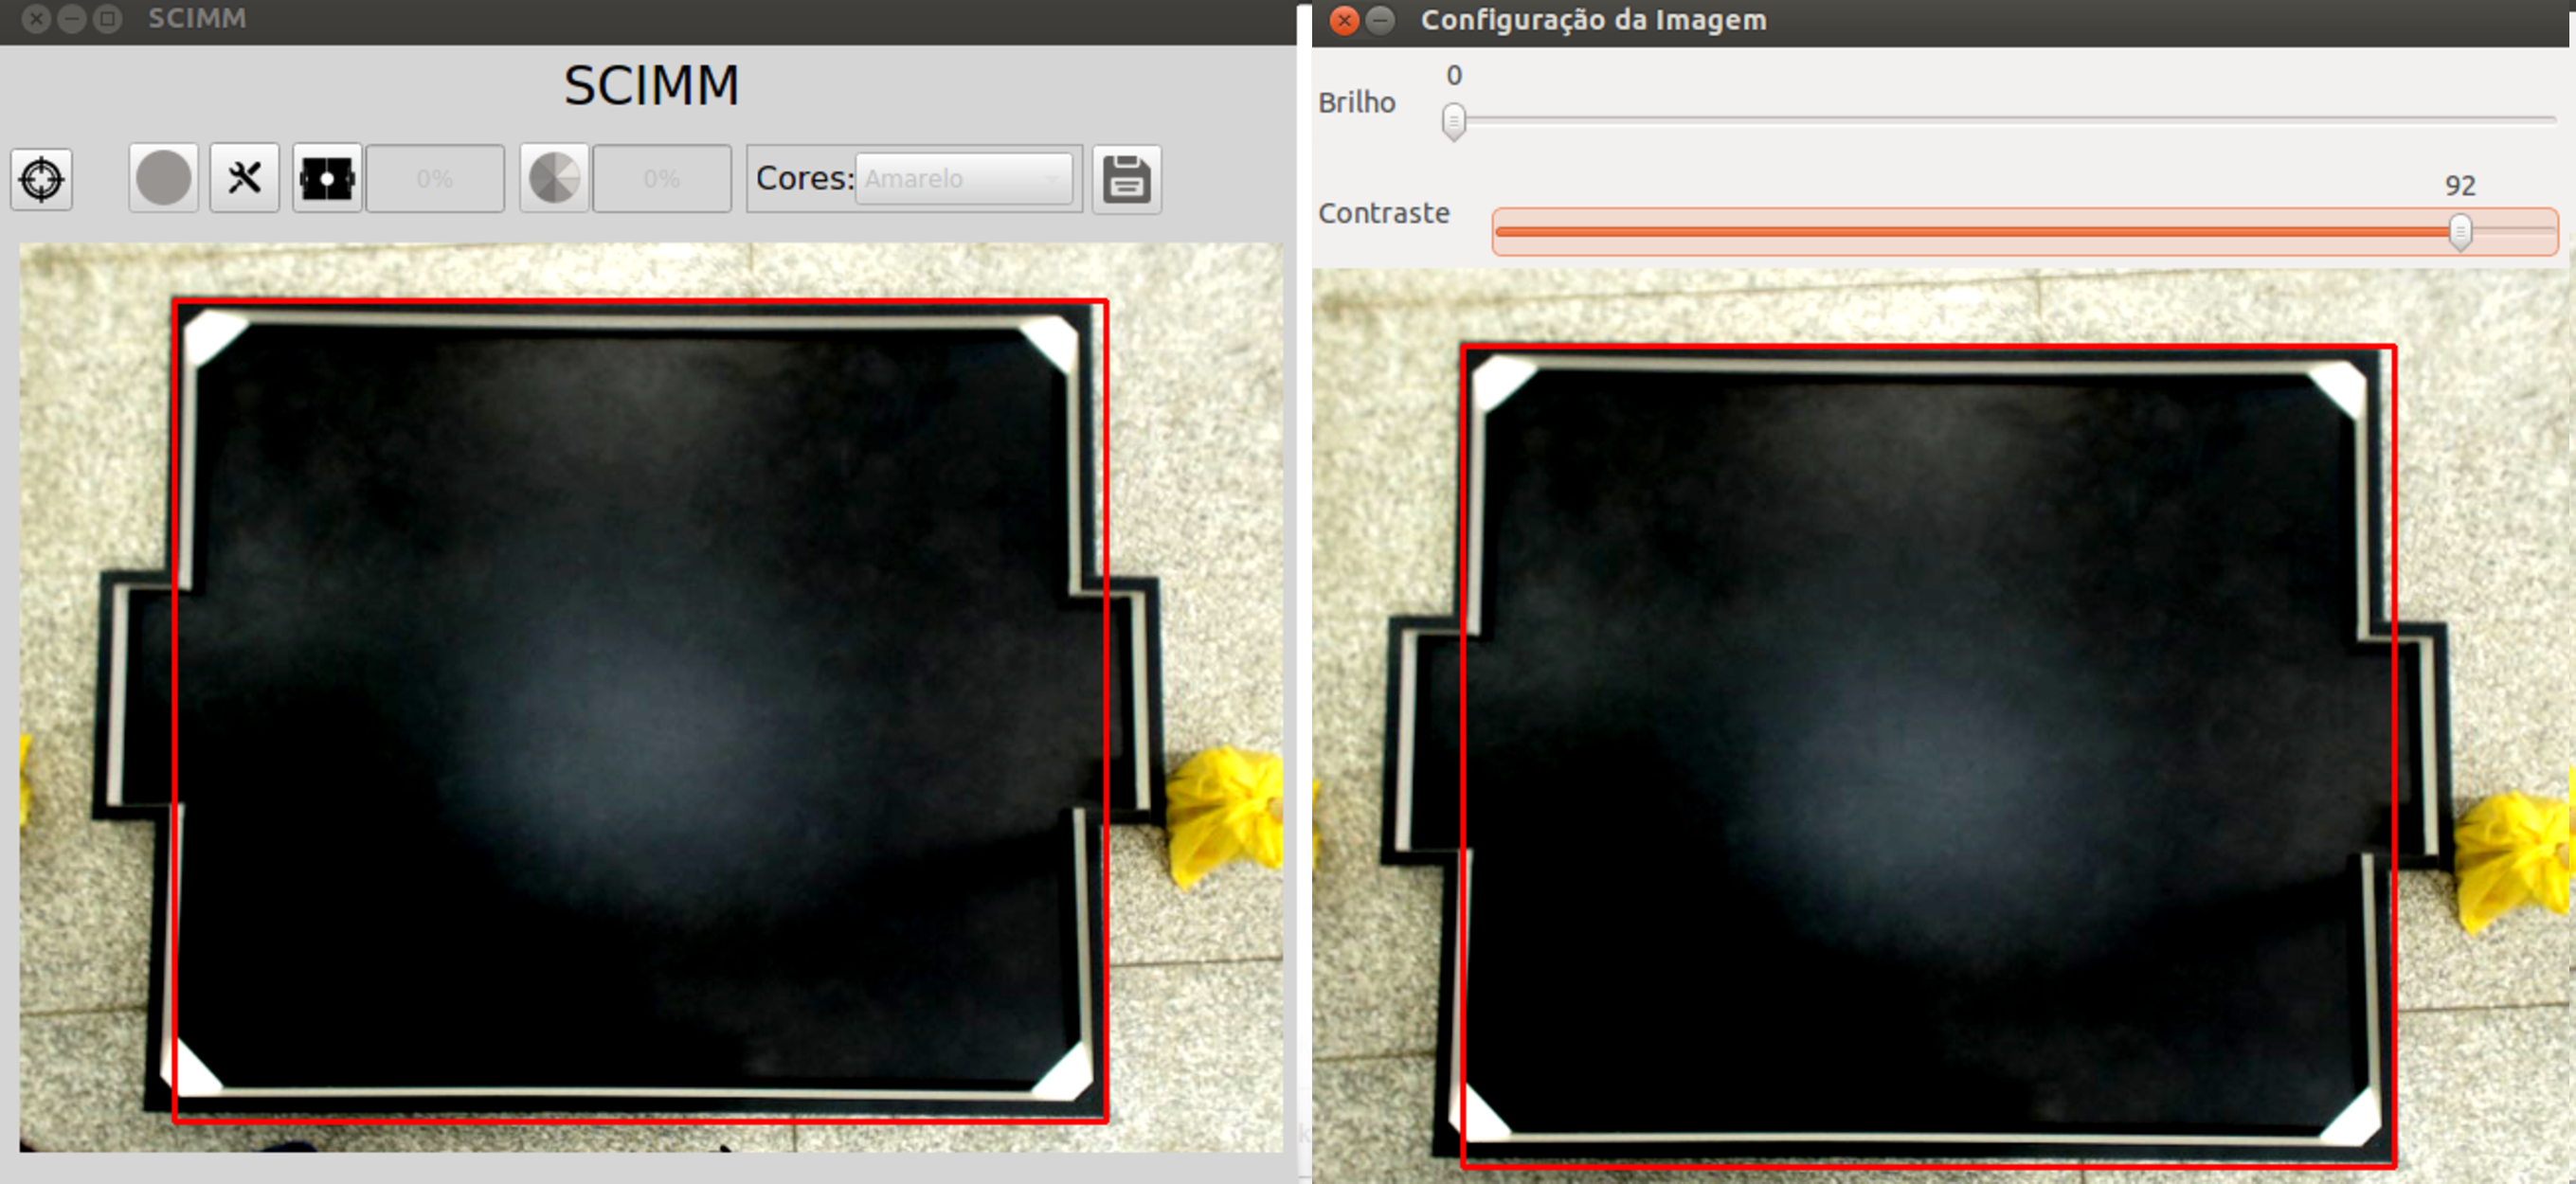
\includegraphics[width=0.8\textwidth]{passo1.pdf}
			\caption{ Configuração de Camera}
			\label{Configuracao}
		\end{figure}		


 Após confirmada a escolha do tamanho da tela 
este é então salvo na variável nomeada \textit{tamanho}, está então sera usado durante todo o processo de calibração.
Além de recorte da imagem, nessa etapa também são configurados Brilho e Contraste de forma que os objetos de cor no campo se tornem mais vividos, se tornando assim também mais nítidos, para que os processos de separação e detecção de objetos sejam mais precisos.	A configuração de Brilho e Contraste utiliza o método \textit{convertTo} da biblioteca \textit{OpenCV} que é utilizada para o melhoramento da imagem antes da detecção dos objetos, a utilização completa fica da seguinte maneira:
\begin{center}
\centering \textit{ frameA.convertTo(frameA, -1, contrast\_value / 50.0, brightness\_value)}
\end{center}
Esta função recebe quatro parametros. O primeiro \textbf{frameA} informa aonde sera salvo o resultado da conversão. O segundo \textbf{-1} indica o tipo da matrix, ou numero de canais, da imagem a ser gerada, usa-se -1 quando se deseja que se use os valores semelhantes aos da imagem da imagem original\cite{OpenCV}, O terceiro \textbf{contrast\_value / 50.0} indica o valor de constraste, ou alpha, a ser usado para multiplicar os valores do pixel da imagem\cite{OpenCV} e por ultimo \textbf{brightness\_value} que é o valor do brilho, ou beta, a ser adicionado à imagem. É importante ressaltar que a configuração de  Brilho e Contraste é somente usada para a melhor precisão na detecção dos objetos, no momento da analise do pixel, a imagem esta \textit{limpa} sem alguma alteração.\newline

	\subsection{2ª Etapa - Reconhecimento de Fundo}
	Um principais problemas que ocorrem na detecção de objetos é a confusão do fundo junto ao próprio objeto, fazendo assim que o mesmo seja detectado porém não seu contorno correto, ou em outras vezes ignorado por ser considerado parte do fundo. Para eliminar este problema foi utilizado a técnica  Subtração do fundo usando Mistura de Gaussianas, por meio do objeto \textit{createBackgroundSubtractorMOG2()} disponível na biblioteca \textit{OpenCV}. Esta técnica utiliza um algoritmo de analise pixel a pixel e que classifica o mesmo baseando-se na distribuição da gaussiana que o representa. Para separar o fundo do resto da imagem é levada em consideração que a gaussiana que representa o fundo tenha grande peso e baixa variância, isso significa que a mesma ocorre frequentemente e varie pouco no tempo. O algoritmo atualiza o modelo de fundo a cada quadro da imagem baseando-se na variância do objetos da mesma e de sua variância. O objeto criado pela biblioteca, por meio do método \textbf{apply}, analisa quadro a quadro a imagem, a compara com o fundo obtido e gera uma imagem chamada de \textbf{máscara} com os objetos que não fazem parte do fundo, no exato momento da imagem, com o passar dos quadros o objeto se torna parte do fundo. Uso do método:
\begin{center}
 \begin{displaymath}  \centering \textit{pMOG2-$\rangle$apply(frame, mask);}  \end{displaymath}

\end{center}

Onde \textbf{frame} significa a imagem atual capturada pela câmera e \textbf{mask} a máscara gerada pela diferença da imagem atual com o modelo de fundo. 

\begin{figure}[H]
			\centering
			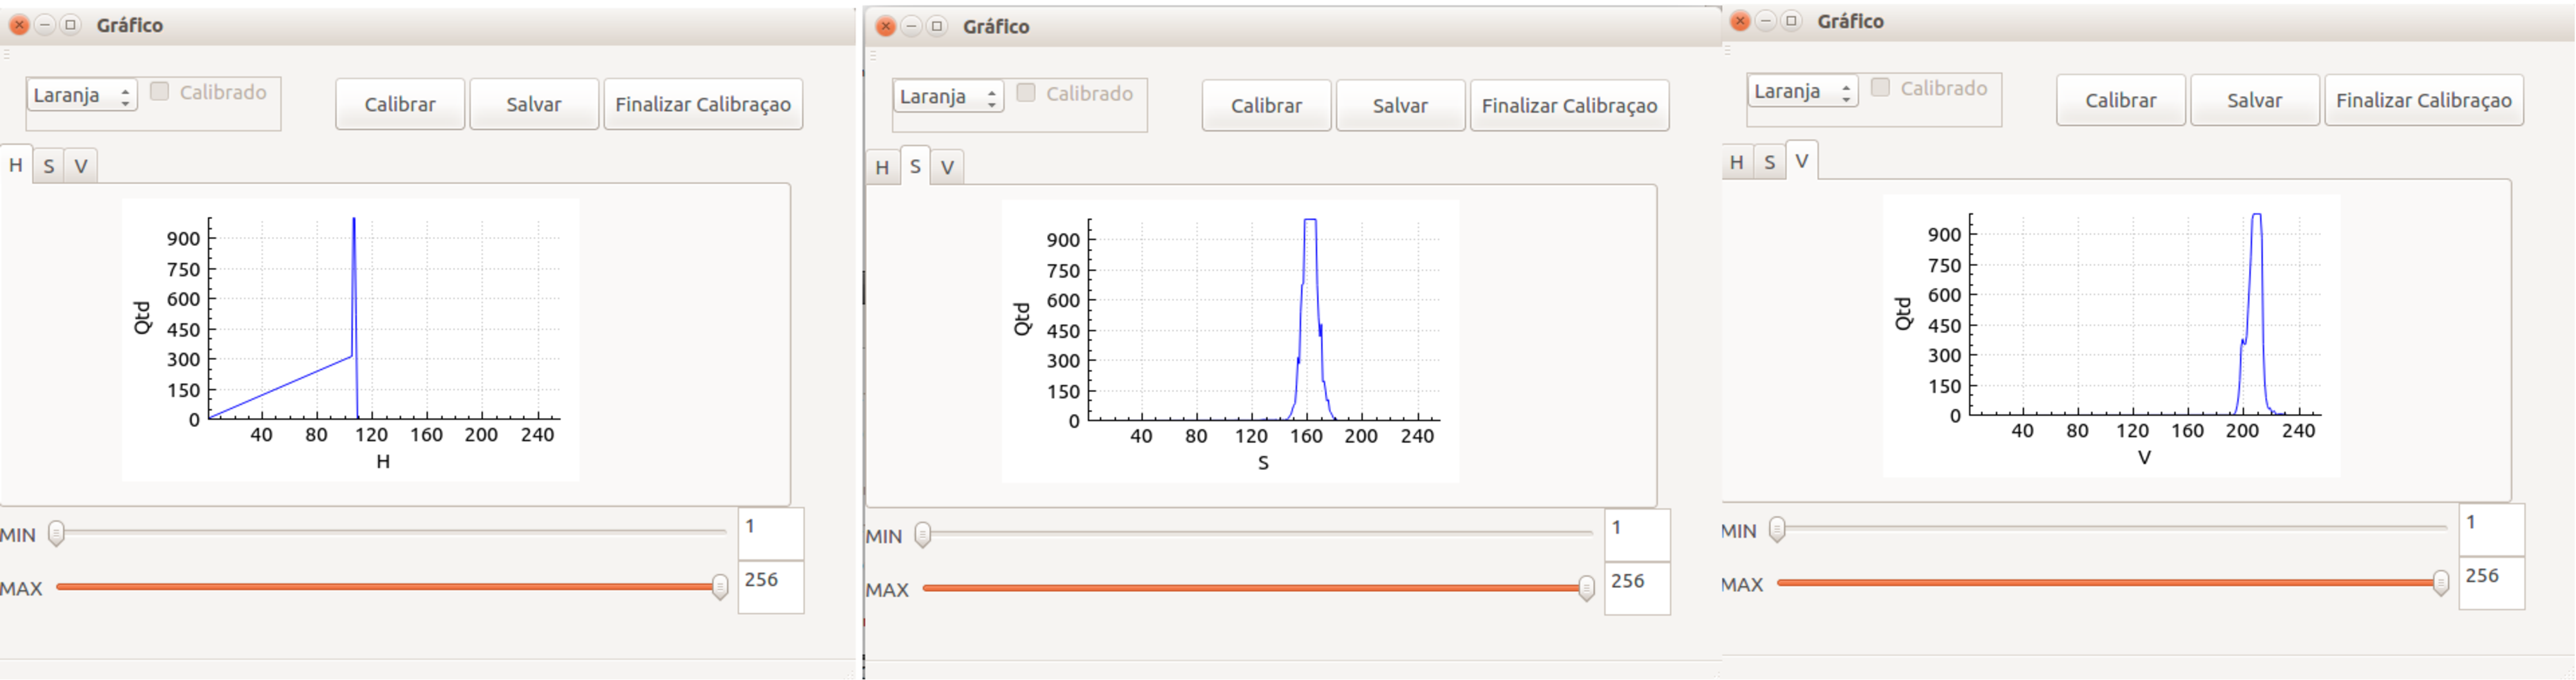
\includegraphics[width=0.45\textwidth]{passo2.pdf}
			\caption{Configuração de Ca mera}
			\label{Configuracao}
		\end{figure}		


Sabendo inicialmente que o modelo de fundo do objeto \textbf{pMOG2} esta vazio, basta que ele seja executado algumas vezes para que o campo se torne o modelo de fundo. Nesse caso a máscara gerada pelo método não chega a ser utilizada, porém sera na 3ª etapa.
	\subsection{3ª Etapa - Extração dos Objetos do Fundo}
	Como visto na 2ª etapa, o objeto \textbf{pMOG2} chamando o método \textit{apply} gera uma máscara de diferença da imagem atual para o modelo de fundo. Sendo assim para obtermos os objetos que virão a ser detectados basta que o método \textit{apply} seja chamado um numero de vezes suficiente para criar a máscara e o mesmo não alterar o modelo de fundo.
	
\begin{figure}[H]
			\centering
			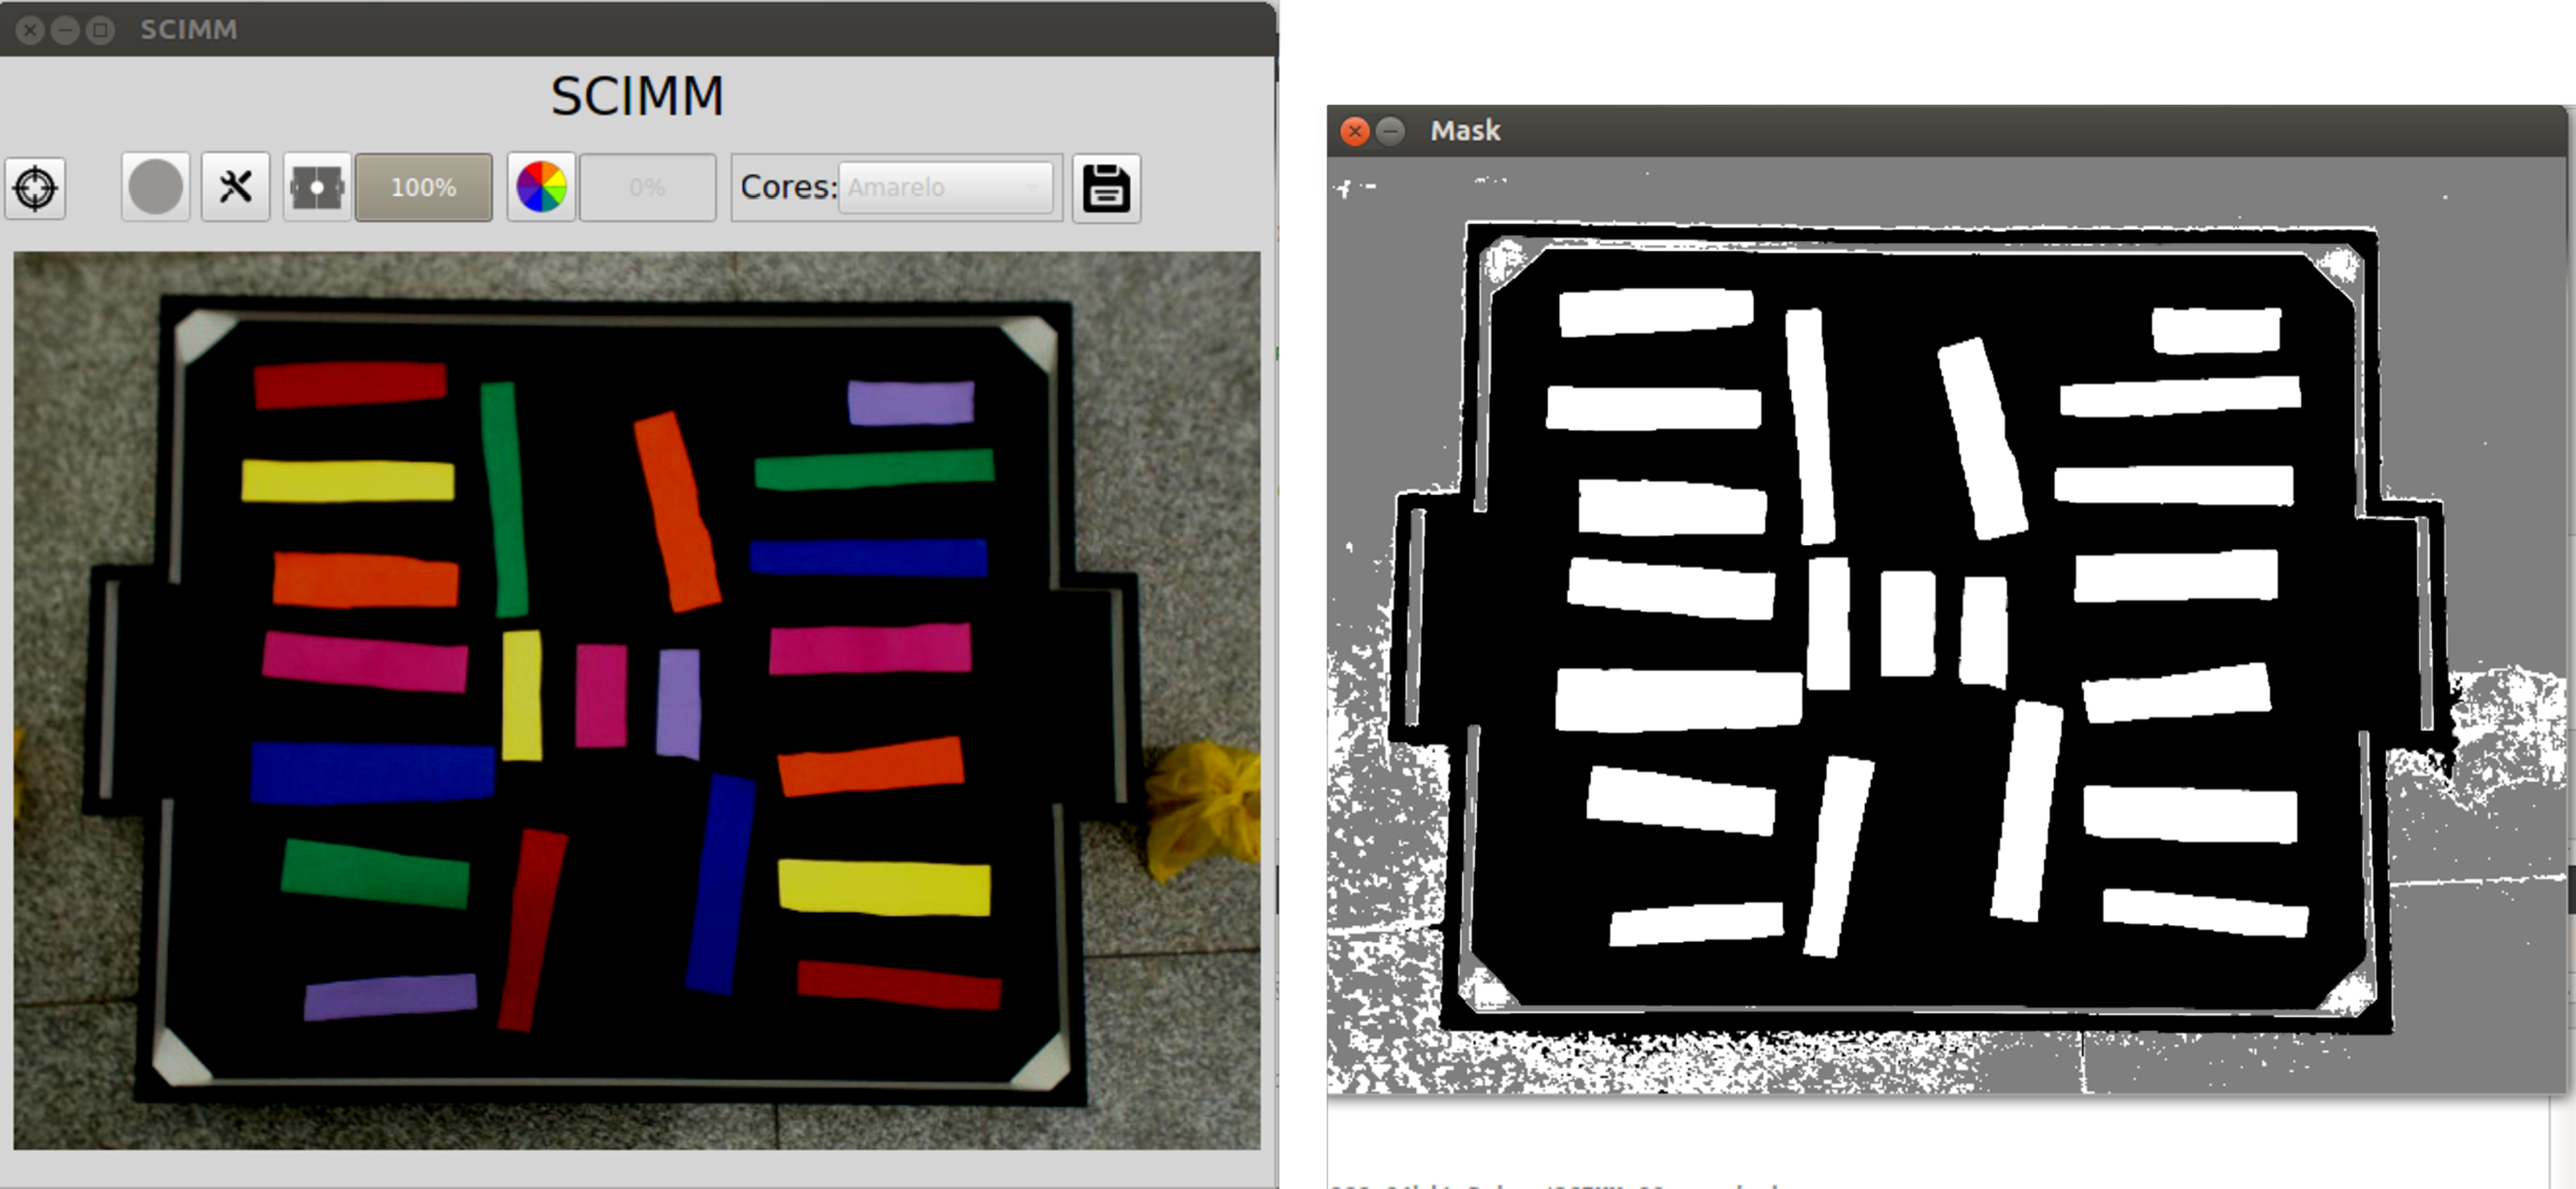
\includegraphics[width=0.8\textwidth]{passo3.pdf}
			\caption{Geração de Máscara}
			\label{Configuracao}
		\end{figure}		


\subsection{4ª Etapa - Detecção e validação de Objetos}
A detecção dos objetos a serem calibrados é dada pelo algoritmo de detecção de bordas de Canny. Como mais um recurso para eliminação de ruídos e melhoria da imagem antes de ser executado a detecção de objetos através da detecção de bordas é utilizado desfoque na imagem. O algoritmo de Canny já está implementado dentro da biblioteca OpenCV e com a seguinte usagem:
\begin{center}
\centering \textit{  Canny(src\_gray, canny\_output, limiar, limiar * 3, 3);}
\end{center}
O algoritmo de Canny utiliza por padrão imagem em padrões de cinza, sendo assim \textbf{src\_gray} é a imagem original transformada para escala de cinza, esta é a imagem na qual o algoritmo sera aplicado. \textbf{canny\_output} será a imagem de saída da função.
\textbf{limiar} e \textbf{limiar*3} são os limites mínimos e máximos para considerar uma borda. \textbf{3} é o valor de apertura ou kernel, o valor 3 é utilizado como padro.

Apos o uso do algoritmo de Canny para detecção de bordas é necessário então fazer uso da função \textit{findContours}, nativa no \textit{OpenCV} para detecção de contornos.
\begin{center}
\centering \textit{ findContours(canny\_output, contours, hierarchy, CV\_RETR\_EXTERNAL, CV\_CHAIN\_APPROX\_SIMPLE, Point(0, 0))}
\end{center}

O primeiro parametro, \textbf{canny\_output}, é a imagem que o algoritmo de Canny gerou com as bordas encontrada na imagem, e é a imagem que o método \textit{findContours} ira utilizar para detectar os contornos, \textbf{contours} é o parametro que indica onde serão salvos os contornos encontrados, cada contorno é armazenado como sendo um vetor de pontos \cite{OpenCV}. \textbf{hierarchy} é onde será salva um vetor de informações sobre a topologia da imagem, e terá como total de elementos o mesmo numero que o total de contornos encontrado\cite{OpenCV}. O quarto parametro, \textbf{CV\_RETR\_EXTERNAL} indica o modo de obtenção de contornos, nesse caso \textit{CV\_RETR\_EXTERNAL} indica que o metodo só obtera os contornos exteriores\cite{OpenCV}. \textbf{CV\_CHAIN\_APPROX\_SIMPLE} indica o metodo que sera usado para aproximação de contornos, o metodo \textit{CV\_CHAIN\_APPROX\_SIMPLE} comprime segmentos horizontais, verticais, diagonais e deixa apenas os seus pontos finais\cite{OpenCV}. E o ultimo parâmetro, \textbf{Point(0, 0)}, indica o valor a ser usado para deslocar a imagem ao encontrar os objetos, neste caso esse valor é 0 para Y e 0 para X, pois não sera necessário. 

Uma vez obtidos os contornos é necessários que se faça a eliminação de vértices dos polígonos encontrados nos objetos deixando assim o objeto mais preciso. Isso é necessário para deixar a forma encontrada mais precisa dá forma original. Para este ajuste foi usado o método \textit{approxPolyDP}, já implementado dentro da biblioteca OpenCV. Esse método teve que ser aplicado em cada um dos contornos encontrados, e foi utilizado da seguinte maneira:
\begin{center}
\centering \textit{    approxPolyDP(Mat(contours[i]), contours\_poly[i], 3, true)}
\end{center}
 Onde o metodo inicia recebendo como paralametro, \textbf{Mat(contours[i])} que é a criação de uma nova imagem, somente com aquele unico objeto, que esta sendo analisado. A seguir é informado no segundo parametro a variavel de destino \textbf{contours\_poly[i]}, onde sera salvo o objeto com a eliminação dos vertices. O terceiro parametro indica o valor do \textit{epilson}, usado o valor \textbf{3} que especifica a precisão da aproximação, a distância máxima entre a curva original e a sua aproximação\cite{OpenCV}. O ultimo parâmetro indica se a curva aproximada sera fechada ou não, foi usado o valor \textbf{true} pois neste caso fechar um uma curva é necessário para que o objeto onde está a cor, seja identificado e analisado na probabilidade.
 Por ultimo os objetos possuem sua borda ignorada, sendo assim calculado o tamanho interior dele, para que por ventura não hajam pixeis de cor preta ou derivadas a serem calculadas.
 
 \subsection{5ª Etapa - Classificação do Pixel}

 
 
 Para que possam ser feita classificação do pixel é necessário que se faça, primeiramente a conversão da imagem obtida pela câmera, normalmente no espaço de cores RGB, para o espaço de cores HSV, pois a mesma lida melhor com diferenças de luminosidade. 
 A biblioteca \textbf{OpenCV} converte o espaço de cor usando a função \textit{cvtColor} que utiliza da imagem original, e de uma imagem vazia com memoria alocada para ser salva a imagem apos a conversão, além do parâmetro do tipo de conversão, Exemplo do uso do método:
\begin{center}
\centering \textit{cvtColor(frame, HSV, CV\_RGB2HSV);}
\end{center}

Apos a conversão é necessário, então, ser feita uma analise dos objetos encontrados. Para cada objeto serão todos os seus pixeis, cada pixel separadamente o mesmo categorizado de acordo com o intervalo de valores ta tabela a baixo:

\begin{table}[h]
\centering
\begin{tabular}{r|r}
Cor & Intervalo de H \\ % Note a separação de col. e a quebra de linhas
\hline                               % para uma linha horizontal
Laranja & de 0 à 20 \\
\hline 
Amarelo & de 21 à 30\\
\hline 
Verde & de 61 à 90 \\
\hline 
Azul& de 91 à 120 \\
\hline 
Roxo & de 125 à 160 \\
\hline 
Rosa & de 161 à 168 \\
\hline 
Vermelha & de 169 à 180 \\
\hline 
\end{tabular}
\caption{Intervalo de Valores de Cores - HSV}
\end{table}

Estes valores foram obtidos através da conversão dos valores de cada cor no universo real para dentro da biblioteca OpenCV. Como visto na sessão 2.2 Cores da fundamentação teórica, o intervalo de valores da matiz(h) é de 0 a 360º graus, porém o valor máximo de armazenamento de um bit é 255, foi incorporada na biblioteca o intervalo de valores de 0 à 180 sendo assim metade do valor do intervalo no mundo real. Uma outra ressalva deve ser feita quando à conversão de valores. O modelo padrão de uma imagem é o RGB, porém dentro da biblioteca espaço padrão é o BGR, quando a imagem é obtida a mesma possui alguns valores invertidos, ou seja, os intervalos de valores da tabela acima podem parecer diferentes do que seria considerado real se forem feitos conversão de valores RGB para HSV. Como não há pre-definição destes valores disponível pela biblioteca, foi feito então testes utilizando os valores considerados no mundo real como base para que chegássemos a esses valores.

Durante o desenvolvimento foi observador que, em sua maioria, as cores necessitavam de um valor S e V pré estabelecido.Para as cores Vermelho, Rosa, Azul, Laranja e Verde foi pré estabelecido o valor de 100 para ambos, S e V, já para Amarelo e Roxo ambos os valores assumem 50.


  \subsection{6ª Etapa - Gerar Arquivo de Cores}
  Assim que todas as cores já estiverem sido assimiladas e a calibração finalizada, gera-se um arquivo chamado \textbf{cores.arff}. 
  
  		
  
  
  

 
 
